\chapter{Evaluation}
\renewcommand{\baselinestretch}{\mystretch}
\label{chap:Eval}
%\setlength{\parindent}{0pt}

\section{\ca{Example sequences}}

\PARstart{\ca{A}}{} \ca{%
few existing sequence designs used for past lighting shows were available for use as example inputs. They all share the same set of output controller configuration. The longest sequence with a mixture of slow and rapid changing effects was used for all subsequent performance analysis, to represent an average complexity of lighting show designs. This sequence lasts for 6 minutes and 49 seconds, has 2900 elements and 8452 output channels.
}

\cmt{Frame difference percentage line chart?}

\section{Original performance}

The original Vixen application already has \ca{a} built-in instrumentation display interface that can show runtime performance figures such as controller update speeds. However, it lacks some elemental functionalities for performance analysis. Data logging, playback timestamps and CPU usage logging were added for performance analysis.

The Vixen application uses a separate thread for each task. It has the main GUI thread for editor, a preview rendering thread and multiple dedicated threads for active controllers. This multi-threading structure can take advantage of modern multi-core multi-thread processors. However, performance on a single core machine can be poor due to context switching. Mutex locks are also required to resolve potential data access conflict, further \ca{increasing} the overhead.

\fref{fig:original} shows the performance of the original Vixen execution engine \ca{on the Microsoft Windows-based platform}. The CPU usage frequently \ca{reached} above $90 \%$, while the refresh rate \ca{was} very unstable around the configured 20 fps. Especially \ca{during} the first 60 seconds, the refresh rate \ca{dropped} to 5 fps while trying to keep up with element updates. At the same time, the CPU usage was \ca{around} $50 \%$. On a dual-core machine, this implies one of the cores was running at full load while the other one was mostly idle.

\begin{figure}[t]
  \centering
  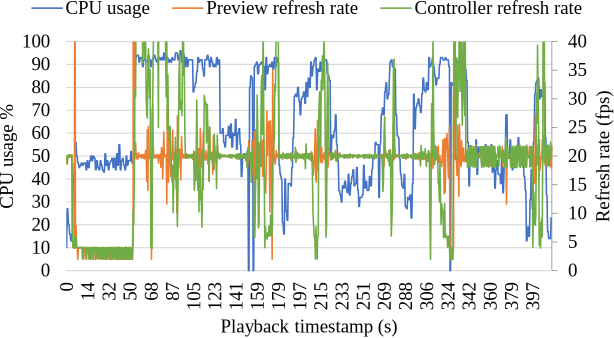
\includegraphics[width=0.8\columnwidth]{original}
  \caption{\footnotesize Performance of original Vixen execution engine}
  \label{fig:original}
\end{figure}

Further analysis using Microsoft Visual Studio's sampling profiler shows, around $24.7 \%$ of total CPU time was \ca{spent} between translation layers for generating controller commands (\texttt{GenerateCommand}), while the actual command assignment (\texttt{\_8BitEvaluator}) \ca{took} less than $0.5 \%$ of CPU time, as shown \ca{in} \fref{fig:vixen_perf_original} \ca{call tree} analysis. Another $23.0 \%$ CPU time was used for filter and element updates, $26.0 \%$ for preview rendering and $16.9 \%$ for the sequence editor, as shown \ca{in} \fref{fig:vixen_perf_original_overview}. The CPU time used for controller updates \ca{was} almost negligible.

\begin{figure}[t]
  \centering
  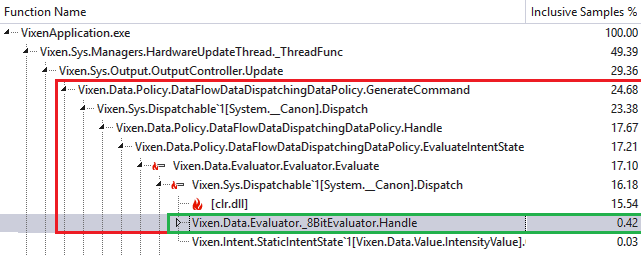
\includegraphics[width=0.85\columnwidth]{Figs/vixen_perf_original.png}
  \caption{\footnotesize \ca{Call tree} analysis of Vixen update threads}
  \label{fig:vixen_perf_original}
\end{figure}

\begin{figure}[t]
  \centering
  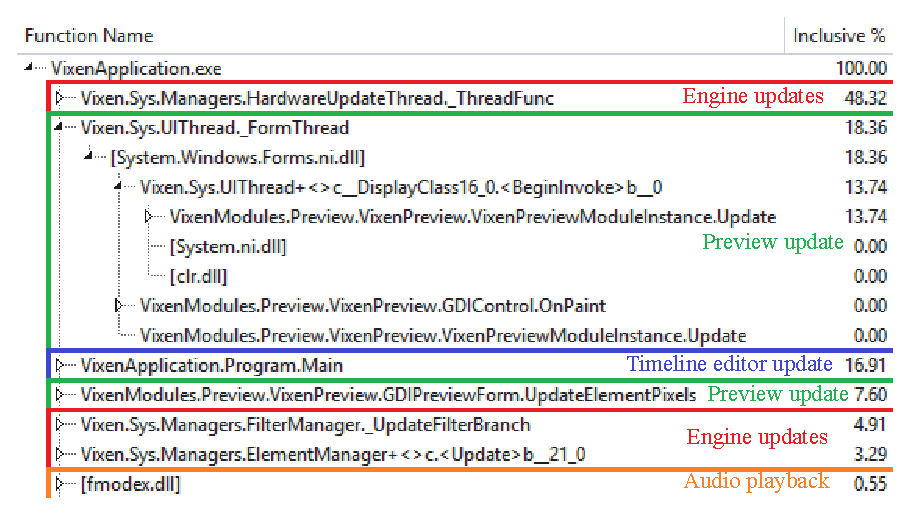
\includegraphics[width=0.85\columnwidth]{Figs/vixen_perf_original_overview.eps}
  \caption{\footnotesize \ca{Call tree} analysis of original Vixen application}
  \label{fig:vixen_perf_original_overview}
\end{figure}

The translation layers are used for determining the actual controller command format. There are several different command formats \ca{for various} controllers. For example, 8-bit, 16-bit or RGB channels. Therefore, the application \ca{needs} to resolve the actual types of commands for specific assignment handlers from a common command base type, which \ca{is} apparently very inefficient in C\#. This process is called \texttt{dispatch} in the source code\ca{;} it must be minimised in order to improve performance.

The implementation of \ca{the} preview display was also very inefficient, \ca{using} only software instance management and sequential rendering. It can be improved by the utilisation of GPU through DirectX or OpenGL.

\ca{To reduce overheads, the show scheduler was used to render the sequences without preview and editor updates. The issue of significant refresh rate drop during first 60 seconds still persists. Although the 20 fps controller became more stabilised later, another 50 fps controller could only reach 40 fps maximum. The CPU usage was mostly around $55 \%$ to $75 \%$. \fref{fig:vixen_perf_original_scheduler} shows the detailed breakdown of CPU time spent for each tasks.}

\begin{figure}[t]
  \centering
  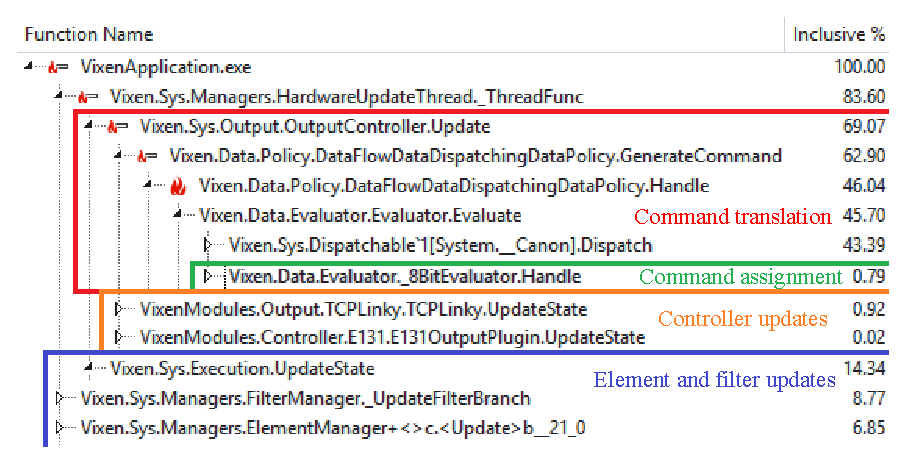
\includegraphics[width=0.85\columnwidth]{Figs/vixen_perf_original_scheduler.eps}
  \caption{\footnotesize \ca{Simplified call tree analysis of Vixen application with reduced overheads}}
  \label{fig:vixen_perf_original_scheduler}
\end{figure}

\ca{Other example sequences were also tested.} They all show similar performance characteristics with unstable playback frame rate for moderately complicated lighting effects.

\section{Port to Linux}

It \ca{took} some necessary modifications for Vixen to run on Linux using mono runtime. The MonoDevelop IDE \cite{monodevelop} \ca{helped} by directly supporting Microsoft Visual Studio projects. However, C/C++ projects were not supported, and pre-built dynamic runtime libraries developed using C/C++ for Microsoft Windows were also not support by mono. All code references to WPF and FMOD audio \ca{had to be} removed for the project to build and run.

The \ca{resulting} Vixen application for Linux has a distorted main GUI with unreasonably long vertical window size. The sequence editor, display setup and preview would either not load or crash the entire application. Fortunately, all controller modules \ca{could} be loaded and the core execution engine and controller update threads were working properly. \fref{fig:vixen_linux_main} shows some loaded controller modules and partially working GUI.

\begin{figure}[t]
  \centering
  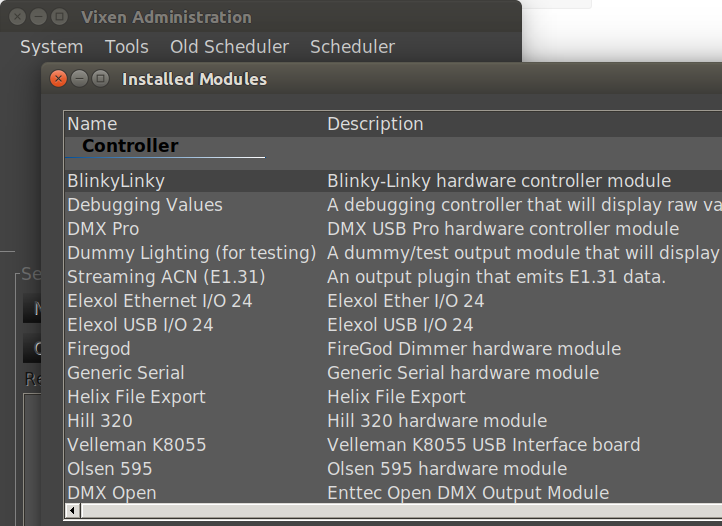
\includegraphics[width=0.8\columnwidth]{Figs/vixen_linux_controllers.png}
  \caption{\footnotesize Controller modules loaded on Linux port of Vixen application}
  \label{fig:vixen_linux_main}
\end{figure}

The intended optimised Vixen application would be command-line user interface (CUI) only with minimal essential functionality. Therefore, the broken GUI should not be an issue\ca{, as GUI related code and modules will not be accessed in the CUI application}.

\section{Extract rendered sequence}

Instead of trying to improve the original execution engine, the performance problem may be eliminated by playing pre-rendered controller layer data frames directly to individual hardware controllers. Channel data type information can be stored separately without the need to resolve through translation layers during runtime. Element updates, Filter updates, \ca{optional GUI updates} are all \ca{unnecessary} for \ca{rendering directly to the controllers}.

Two steps are needed for this approach. \ca{The sequence must be pre-rendered} with precise frame interval, then \ca{the rendered data must be played back} to the controllers as a separate process\ca{, possibly} on an entirely different platform.

To pre-render the sequence, two different methods are possible. A dummy controller can be used for runtime data dumping, or a separate export engine with manual frame control independent of wall-clock time \ca{can be used}. \ca{Both of these methods were tested. Although a custom controller fit more naturally and requires less modification to the existing structure, it cannot give the indication of sequence start, end and information about other controllers. More importantly, it can have unstable frame rates influenced by CPU usage. A high performance computer is required for near prefect pre-rendering by controller dumping. Therefore, the existing sequence export function from sequence editor was used instead.}

\section{Custom controller}
\label{sec:tcplinky}

A custom controller module (\texttt{TCPLinky}) was developed based on one of \ca{Vixen's} existing \ca{controllers} (\texttt{BlinkyLinky}). This controller uses TCP connection to transfer display channel data, \ca{and} supports up to 65535 channels. A corresponding cross-platform server application that simulates a multi-channel display was also developed using C++ with Qt \cite{qt} and OpenGL \cite{shreiner2009opengl} rendering. \ca{This combination of programming language and GUI libraries enables fast packet decoding and GPU acceleration for display interface,} allows real-time \ca{simulation of numerous display output channels} without the need \ca{for} a complex physical lighting system setup. Data dumping, performance and statistical analysis can also be easily achieved.

\fref{fig:tcplinky_server} shows a screenshot of the server application. \cad{With the help of GPU...} \ca{On the Windows-based testing platform,} it consumes less than $3 \%$ of CPU time under 50 fps refresh rate, which is negligible. It \ca{was also} compiled and executed on other computers \ca{to simulate real-world} network connected controller scenarios. \ca{For  all performance tests performed in this project, this server application was running on a platform different to the platform under test, in order to reduce undesired impact of performance and simulate controller connection.}

\begin{figure}[t]
  \centering
  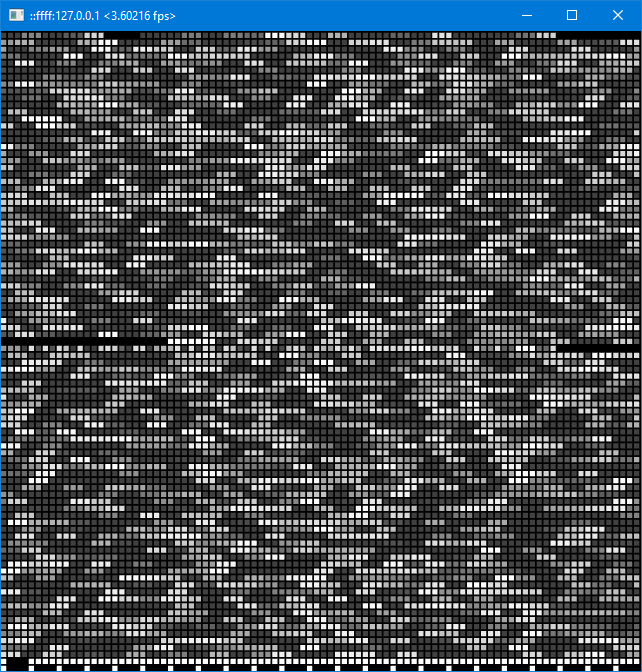
\includegraphics[width=0.6\columnwidth]{Figs/tcplinky_server.png}
  \caption{\footnotesize Screenshot of \texttt{TCPLinky} controller server application}
  \label{fig:tcplinky_server}
\end{figure}

The reference controller implementation \texttt{BlinkyLinky} skips sending data packets when no data change \ca{is} detected. However, this is not desired for performance analysis. Therefore, this mechanism was bypassed by the \texttt{TCPLinky} controller. Data packets will be sent regardless of whether data changes \ca{are} detected or not.

\ca{To avoid losing configurations of previously defined controllers, this controller was patched in parallel with existing controllers. This resulted in a duplication of channels in the exported sequences, as different controllers map to different frame data segments.}

\section{\ca{Sequence exporting}}

\cad{Although the custom controller module is capable of...}

\ca{The existing sequence export function from sequence editor} was originally used to convert the lighting sequence to formats recognisable by other controller specific applications. It renders the sequence using a manual timing source stepped after each frame, \ca{giving} accurate constant data dump intervals. It can also write all controller channel mapping information to a separate XML file. An example XML file is shown \ca{in} \lref{lst:network_xml}.

\begin{lstlisting}[float,floatplacement=ht,language=XML,label=lst:network_xml,captionpos=b,caption={\footnotesize Example controller mapping XML file}]
<?xml version="1.0" encoding="utf-8"?>
<Vixen3_Export>
  <Resolution>20</Resolution>
  <OutFile>luf2013_20ms.raw</OutFile>
  <Duration>00:04:45.8050000</Duration>
  <Network>
    <Controller>
      <Index>0</Index>
      <Name>E6804 arches L</Name>
      <StartChan>1</StartChan>
      <Channels>2048</Channels>
    </Controller>
    <Controller>
      <Index>1</Index>
      <Name>Lynx DMX</Name>
      <StartChan>2049</StartChan>
      <Channels>156</Channels>
    </Controller>
  </Network>
  <Media>
    <FilePath>example_audio.mp3</FilePath>
  </Media>
</Vixen3_Export>
\end{lstlisting}

To support the \ca{proposed} optimised playback engine, audio media file path was added to the XML. The export dialog window was modified to allow custom frame resolution through text input, instead of a few pre-defined fixed values on the drop down list, as shown \ca{in} \fref{fig:vixen_export}. \ca{An additional} data format \ca{entry named ``Raw File''} for the playback engine was also added to the export wizard. This ``Raw'' format is a simple sequential concatenation of frames, where each frame \ca{comprises} of 6-byte header, 2-byte channel count and \ca{is} followed by continuous channel data.

\begin{figure}[t]
  \centering
  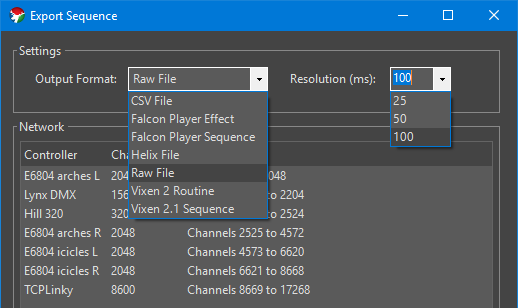
\includegraphics[width=0.75\columnwidth]{Figs/vixen_export.png}
  \caption{\footnotesize Modified Vixen export dialog window}
  \label{fig:vixen_export}
\end{figure}

\ca{The example sequences were exported using 20 ms interval, or 50 fps. Because of the lack of hardware lighting setup, only the \texttt{TCPLinky} controller running at 50 fps was enabled for output. The exported channels were still duplicated, resulted in a total of 17268 channels for each frame, including 8600 channels for the \texttt{TCPLinky} controller.}
